\documentclass[10pt]{article}

\usepackage{amsmath}

\numberwithin{equation}{section}

\usepackage[english]{babel}
\usepackage[utf8]{inputenc}
\usepackage{amsfonts}
\usepackage{graphicx}
\usepackage{epstopdf}
\usepackage{caption}
\usepackage{float}
\usepackage{bm}
\usepackage{esvect}
\usepackage{hyperref}
\usepackage{listings}

\usepackage{setspace}
\onehalfspacing

\oddsidemargin = -5pt
\evensidemargin = -5pt
\textwidth = 500pt
\topmargin = -50pt
\textheight = 650pt

\title{SPM Report}
\date{}
\author{
	Massimo Equi\\
	AY 2017/2018
}

\begin{document}
\maketitle

\section{Introduction}  \label{intro}
The chosen project is the one consisting in using a genetic algorithm to estimate an unknown function $f$ given a set of pairs $\left(x, f\left(x\right)\right)$ as input.

\section{User Manual} \label{usermanual}
In order to compile and run the program follow these instructions:
\begin{itemize}
\item move to the \verb|SPM_FinalProject| directory;
\item if needed, run the command \verb|make clean|, it will remove all the \verb|.o| and \verb|.out| files; 
\item compile the program with the command \verb|make -f [makefile]|
\item run the sequential program with \verb|./main.out [parameters] < [input_file]|
\item run the parallel program with \verb|./parallel_main.out [parameters] < [input_file]|
Here it is an example of a typical session:
\begin{verbatim}
$ make clean
$ make -f Makefile.icc
$ make -f Makefile.ff.icc
$ make -f Makefile.thread.icc
$ ./main.out 12000 5 4000 10 20 0.5 no < input_cos\(x\)-pow\(x,3\)10-3.txt
$ ./ff_main.out 12000 5 4000 10 20 0.5 8 no < input_cos\(x\)-pow\(x,3\)10-3.txt
$ ./thread_main.out 12000 5 4000 10 20 0.5 8 no < input_cos\(x\)-pow\(x,3\)10-3.txt
\end{verbatim}
\paragraph{Makefile}
For compiling the sequential program, \verb|[makefile]| can be one of the following:
\begin{itemize}
	\item \verb|-f Makefile| (or simply \verb|make|) compiles the program with the \verb|g++| compiler;
	\item \verb|-f Makefile.icc| compiles the program with the \verb|icc| compiler;
	\item \verb|-f Makefile.icc.mic| compiles the program with the \verb|icc| compiler using the flag \verb|-mmic|;
\end{itemize}
All of the above commands output a \verb|main.out| file.\\
For compiling the FastFlow version of the program, \verb|[makefile]| can be one of the following:
\begin{itemize}
	\item \verb|make -f Makefile.ff| compiles the program with the \verb|g++| compiler;
	\item \verb|make -f Makefile.ff.icc| compiles the program with the \verb|icc| compiler;
	\item \verb|make -f Makefile.ff.icc.mic| compiles the program with the \verb|icc| compiler using the flag \verb|-mmic|;
\end{itemize}
All of the above commands output a \verb|ff_main.out| file.
For compiling the version of the program that uses threads, \verb|[makefile]| can be one of the following:
\begin{itemize}
	\item \verb|make -f Makefile.thread| compiles the program with the \verb|g++| compiler;
	\item \verb|make -f Makefile.thread.icc| compiles the program with the \verb|icc| compiler;
	\item \verb|make -f Makefile.thread.icc.mic| compiles the program with the \verb|icc| compiler using the flag \verb|-mmic|;
\end{itemize}
All of the above commands output a \verb|thread_main.out| file.
\paragraph{Run the program}
The program runs with several parameters and has to be called with and input file. Calling \verb|./main.out|, \verb|./ff_main.out| or \verb|./thread_main.out| with no arguments will show a quick guide. \verb|[parameters]| consists in the following: 
\begin{itemize}
	\item \verb|tree_no| is the number of trees that will be created in the random pool generated at the beginning of every execution;
	\item \verb|depthmax| is the maximum possible depth a tree in the pool can have;
	\item \verb|threshold| is the number of trees the algorithm will select to generate the next population (has to be lesser than \verb|tree_no|);
	\item \verb|randmax| is the largest value a leaf of a tree holding a constant can have;
	\item \verb|gen_no| is the number of generations such that, once reached, the algorithm will terminate;
	\item \verb|err| is the threshold for the fitness. If the fitness of the best tree is lesser that \verb|err| the program will terminate; if \verb|err| is a negative number the algorithm will stop only after reaching \verb|gen_no| generations;
	\item \verb|nw| is the number of parallel workers (skip this argument if the program is sequential);
	\item \verb|debug| can be either \verb|yes| or \verb|no|; if it is \verb|yes| it runs the program with detailed information at each generation.	   
\end{itemize}
The program requires an input file to run. Any file in this project's root directory whose name begins with the string \verb|input_| is a legal input file. In all the executions mentioned in this report we used the input file \verb|input_cos(x)-pow(x,3)10-3.txt| (\verb|10-3| in the name of the file means there are $10^3$ input pairs $(x,f(x))$ in that file).\\
After having compiled the main program, the command \verb|make [makefile] test| can be used to generate \verb|test_FitnessTime.out|. This little test program can be executed specifying an input file (and no arguments) in order to get some estimations about the time needed to evaluate a tree and compute the fitness function.
\end{itemize}

\section{Structure of the code} \label{codestructure}
The code has two main directories: \verb|src/| is where the \verb|.cpp| source files are located while \verb|include/| is where the \verb|.h| header files can be found. Both \verb|src/| and \verb|include/| are structured in three subdirectories: \verb|grammar/|, \verb|genetics/| and \verb|main/|.

\paragraph{grammar}
In \verb|grammar/| there are all the classes needed to implement the grammar provided in the project assignment. Every class is implementing a nonterminal symbol of the grammar with methods that allows it to be expanded using one of its production. The nonterminal \verb|<unop>| and \verb|<binop>| are directly encapsulated in the class \verb|Node| which of course implement the nonterminal \verb|<node>|. Each of these classes gives a concrete implementation of the abstract class \verb|INode|, which is meant to represent a generic node in the syntax tree. An object of class \verb|Node| can be randomly expanded to a given depth using the method \verb|Node::expandRandom()|. Finally, the parameter \verb|randmax| gives and upper bound to the highest number that the class \verb|Const| can store.

\paragraph{genetics}
In \verb|genetics/| the class \verb|Tree| is implementing the behavior of a syntax tree meant to represent a function. Basically, \verb|Tree| provides a nice interface to store and manage the root node of this syntax tree. The class \verb|Forest| is the core of the algorithm since it manages a pool of \verb|Tree|s providing methods to perform mutation and crossover over them. The two classes \verb|FF_Forest| and \verb|ThreadForest| are subclasses of \verb|Forest| and they are used to override the part of the code that was chosen to be turned from sequential to parallel.

\paragraph{main}
In \verb|main/| the file \verb|evolution_cyle.hpp| uses a \verb|Forest| to implement the genetic algorithm. \verb|main.cpp|, \verb|ff_main.cpp| and \verb|ff_main.cpp| call \verb|evolution_cycle.hpp| passing it respectively a \verb|Forest|, a \verb|FF_Forest| or a \verb|ThreadForest|.

\section{Parallelization Choices}
\subsection{Decomposition Strategy}
The main operations that our algorithm is performing are: \emph{selection}, \emph{mutation} and \emph{crossover}, \emph{replication}. Running the sequential version of the program we see that the completion time of \emph{selection} is usually at least one order of magnitude larger than the one needed for \emph{replication}, \emph{mutation} and \emph{crossover}. For this reason, we focused on optimizing only the \emph{selection} phase. Moreover, try to parallelize \emph{mutation} and \emph{crossover} would lead to two major issues. First, the logic of the program would change and hence the accuracy too because parallelize \emph{crossover} means assign to each worker a portion of the array storing the best trees to avoid any synchronization delay; this would imply perform \emph{crossover} among only a portion of the best trees instead all of them. Second, since \emph{mutation} and \emph{crossover} affects only the bet \verb|threashold| trees, we will work in parallel on a set of trees that is much smaller than the entire pool, leading to not parallelization advantages eventually non relevant. Finally, we also decided to not parallelize the \emph{replication} part because the amount of work we would do for a single tree would be too little (just copying the tree itself) due to the fact that the trees that are more likely to be reproduced are the shallower.\\
Focusing on \emph{selection} and analyzing the structure of the problem we observe that it is embarrassingly parallel at two different level of grain. At each iteration our program has to compute the fitness function of all the trees in our pool, hence for every of those trees it is required to evaluate the function that tree is representing over all input data points. This means we could parallelize:
\begin{itemize}
	\item at a \textbf{fine grain} level, evaluating in parallel the function represented by a single tree over different data points;
	\item at a \textbf{coarse grain} level, computing in parallel the fitness function for different trees.
\end{itemize}
Therefore, the first thing we have to discuss if it is worth it to parallelize at any of this two levels of grain.
\paragraph{Single tree parallelization}
In a typical execution of the code we have to handle trees whose depth is set to be not greater that $8$. This is because most of the times the best trees tent to be the shallower ones hence it is useless to set a very high depth since the deeper trees most probably will be discarded soon. Moreover, the average depth is usually smaller than $3$; this means that on the average we perform $2^{3+1}-1=15$ floating point operations per tree, assuming a floating point operation per node. This means that the amount of time we spend evaluating a tree has roughly at most $10^{-1}\mu$$s$ order of magnitude. If we compare this with the time spent to create a thread (approximately $10\mu$$s$) we realize that even if every worker of our hypothetical parallel computation processed $100$ input points this would still be comparable with the effort needed to set up the thread for that worker, hence at least $1000$ input points per thread are needed to have a reasonable advantage. Therefore, if for instance we supposed to work with $10$ workers, we would need more that $10^{4}$ input points to get any advantage from the parallelization, and this would rarely be the case. This is clearly a scenario where we would have a very poor scalability. Thus, we conclude claiming that it is not worth it to parallelize the program relaying on such a fine grain.
\paragraph{Pool parallelization}
Considering instead the whole pool of trees the workload that would be assigned to a worker in a parallel computation is reasonably large and, more importantly, increases easily with the input size. The fitness function for a tree is computed in order of $10^{2}\mu$$s$, hence having only $10$ trees per worker is already enough to get a workload of $10^{3}\mu$$s$. Typically we work with a pool consisting of thousands of trees and this usually means that every worker will have order of $10^{2}$ trees to handle, even in situations with hundreds of parallel workers. Hence we conclude that is worth it to parallelize at this level of grain.

\subsection{Implementation of the Parallel Part of the Code}
The difference between the sequential and the parallel version of the code resides in the classes \verb|FF_Forest| and \verb|ThreadForest|. The class \verb|FF_Forest| uses a FastFlow \verb|ParallelFor| object to manage the workers needed to compute the fitness functions in parallel. The \verb|C++| sequential \verb|for| loop present in the \verb|Forest| class is replaced by a call to the FastFlow method \verb|parallel_for()|. We could use a parallel for due to the fact that no synchronization is needed among the various iterations of the loop since computing the fitness function resembles the \emph{map} pattern. The same reasoning applies in the \verb|ThreadForest| case, where instead of a parallel for we create a thread for each one of the workers passing them the starting and ending positions of the pool at within which they have to work. We leave the main thread waiting for the termination of the others. We are aware we could use a barrier and reuse the same threads at each iteration but this would have complicated a lot the logic of the code. After the \emph{selection} phase, one thread would have had to continue the execution to perform \emph{mutation}, \emph{crossover} ans \emph{replication} while all the others would have had to wait until the beginning of the next iteration, not letting us to use the standard barrier programming pattern. We estimate that the effort needed to create a thread (order of microseconds) is reasonably negligible if compared to the amount of work that thread will do (order of milliseconds), hence we have chosen the aforementioned implementation solution.

\section{Expected Results}
In our scenario we have parallelized our code using a farm pattern whose overheads resides mostly on splitting the initial task in several subtasks and assigning them to different parallel executors. This splitting-and-assigning phase has to be performed at the beginning of each iteration of the evolution cycle. Even if this could potentially lead to a meaningful overhead, there is another problem that will lead to bad performances in terms of \emph{speedup}, \emph{scalability} and \emph{efficiency}. In fact, the sequential part of the code, and in particular the \emph{replication} phase (that we decided not to parallelize for the reasons already explained), have quite a lot of work to do since it is needed to go through all the positions in the array to populate the pool that will be used at the next iteration. If we are using a array with thousands of entries this effort could be relevant. Hence we do not expect to be able to almost halve the completion time with only $2$ workers. We estimate to have such result with $4$ or $6$ workers and to almost achieve the best completion time with $10$ to $12$ workers. As a consequence, we expect to have a speed up closer to the ideal one using up to $6$ workers and then to have it grow slower.For the Xeon PHI machine we could have another problem: since the clock speed is lower we have to use a way smaller input size. This could easily in a loss in terms of scalability due to a too little workload per worker when using lots of cores.\\
For what regarding the performances between the two parallel implementations, we expect the thread implementation go a bit worse when using a large number of workers since it would suffer from the fact that it has to instantiate the threads at each iteration. Nevertheless, we do not expect to have very different performances since, as explained earlier, the amount of work per thread should counterbalance their creation cost.

\section{Achieved Results}
Here we report the actual \emph{completion times} we measured on the Xeon CPU E-2650 and the Xeon PHI machines for the parallel executions of the program, alongside with the graphs for the \emph{speedup}, \emph{scalability} and \emph{efficiency}, comparing these results with the sequential program's ones. The \verb|err| parameter has been always set to \verb|-1| in order to perform exactly \verb|gen_no| iterations; we would not have been able to have comparable results otherwise.
\paragraph{Format of the results}
The program uses \verb|std::chrono| statements in order to output the time spent to perform the computation. We stored all the results in two files: the file \verb|tests| for the Xeon machine and the file \verb|tests.phi| for the Xeon PHI machine. Both files has a line storing the output of the \verb|uptime| command in order to record the state of the machine at the execution time. Each one of the lines storing the results of the tests starts with the string \verb|results|, hence you can get the list of all the outputs with the command \verb|grep results tests[.phi]|. \verb|tests| has been produced recording the output on the shell via a \verb|script| command while for \verb|tests.phi| we just used output redirection (since there is no command \verb|script| on the Xeon PHI). The scripts \verb|test.sh| and \verb|test.phi.sh| run all the tests from scratch (without recording them by their own), but this requires a huge amount of time and we think it will not be needed.
\paragraph{Gathering the results}
We used this parameter setting for all the execution (of course, no \verb|nw| parameter was needed for the sequential execution). For the \textbf{Xeon} we had:
\begin{verbatim}
	tree_no = 12000; depthmax = 5; threshold = 4000;
	randmax = 10; gen_no = 20; err = -1;
	nw = [1, 2, 4, 6, 8, 10, 12, 14, 16];
\end{verbatim}
while for the \textbf{Xeon PHI} we had:
\begin{verbatim}
tree_no = 2400; depthmax = 5; threshold = 800;
randmax = 10; gen_no = 20; err = -1;
nw = [1, 10, 20, 30, 40, 50, 60, 70, 80, 90, 100, 110, 120].
\end{verbatim}
We passed \verb|input_cos(x)-pow(x,3)10-3.txt| as input file, hence we had $1000$ input pairs $(x, f(x))$. As previously stated, the smaller number of trees on the Xeon PHI is due to the lower clock speed. We performed $7$ runs of the program for every parameter setting, we took out the the minimum and maximum time and then we computed the average of the remaining.

\subsection{Xeon}
Taking a look at the graph for the speedup in \figurename~\ref{fig:xeonspeedup} we can conclude that we have performances not as good as expected. We needed $8$ parallel executors just to halve the completion time. We can conclude that the sequential part of the program played a major role in not letting us get good results in terms of speedup and indeed we notice that the efficiency fall down quickly as the number of parallel executors grows. Taking a look at the scalability we notice that the thread implementation stays above the FastFlow one. This is because, if the workload per thread is large, using only few of them significantly slow down the computation. This leads to better improvements when using more workers than in the FastFlow case, which is able to handle more efficiently the case of one worker not creating it at every iteration.

\subsection{Xeon PHI}
Even in this case we experience the same issues as for the Xeon. As expected, we got good results using up to $10$ workers, with limited improvements using a larger number of them. As mentioned before, one problem here was probably not being able to use a input size large enough due to the overall completion time of the tests. Most probably the running time of the parallel part of the code becomes comparable with the one of the sequential part already using $10$ workers, leaving no room for significantly better performances even with more workers. Nevertheless, \figurename~\ref{fig:xeonphispeedup10} shows that, despite the performances that we got for the Xeon, here the speedup is growing in a natural way (using up to $10$ workers). This could mean that the difference between the time spent to perform floating point operations and standard logical operation on the Xeon PHI is higher than the one on the Xeon. In this case the \emph{selection} phase would take a so much longer time than the others that it would be enough to make negligible the effort spent in the sequential part of the code. This would also explain why we got so similar performances between the FastFlow implementation and the thread implementation: spending most of the time performing floating points operations makes the overheads of creating threads less significant.
\begin{figure} 
	\centering
	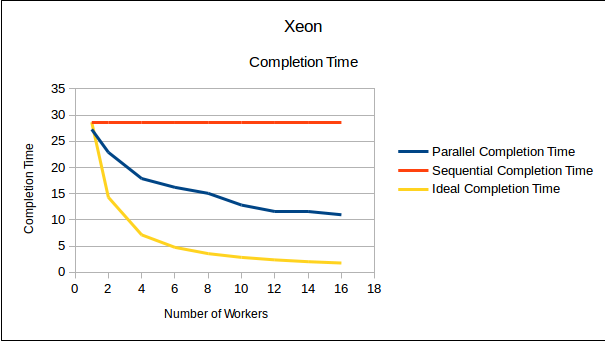
\includegraphics[scale=.75]{Xeon_CompletionTime.png}
	\caption{Completion time on the Xeon.}
	\label{fig:xeoncompletiontime}
\end{figure}

\begin{figure} 
	\centering
	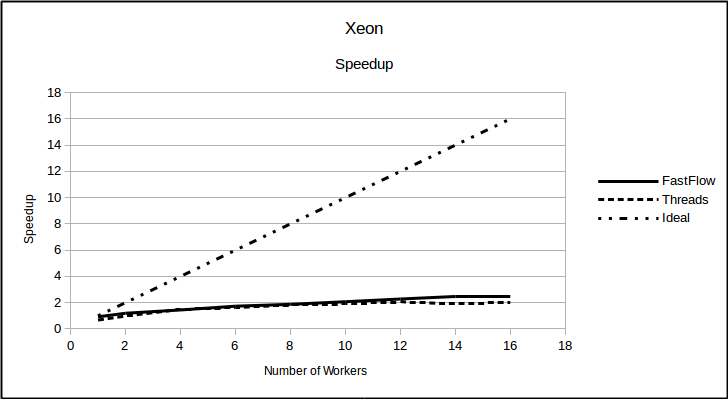
\includegraphics[scale=.75]{Xeon_Speedup.png}
	\caption{Speedup on the Xeon.}
	\label{fig:xeonspeedup}
\end{figure}

\begin{figure} 
\centering
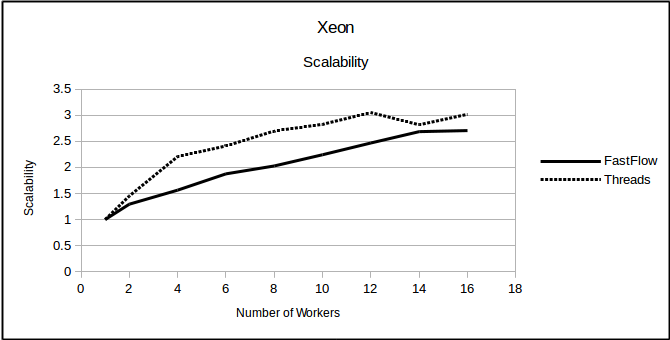
\includegraphics[scale=.75]{Xeon_Scalability.png}
\caption{Scalability on the Xeon.}
\label{fig:xeonscalability}
\end{figure}

\begin{figure} 
\centering
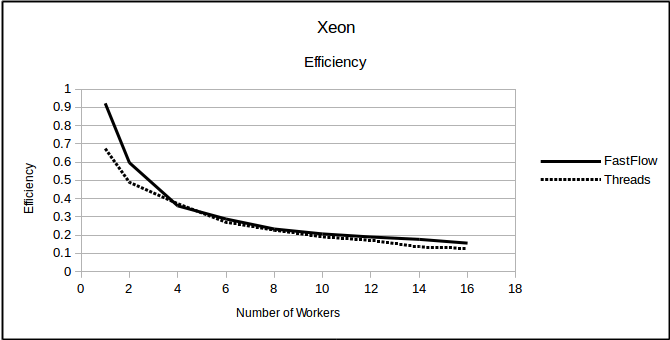
\includegraphics[scale=.75]{Xeon_Efficiency.png}
\caption{Efficiency on the Xeon.}
\label{fig:xeonefficiency}
\end{figure}

\begin{figure} 
	\centering
	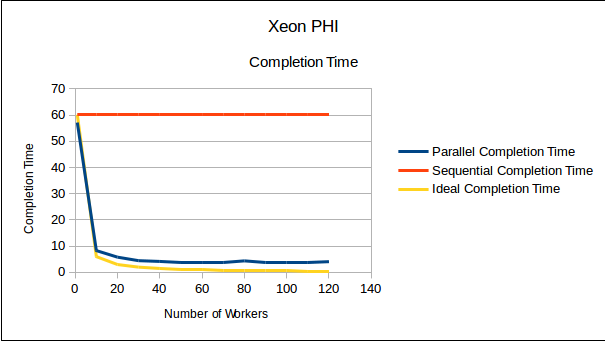
\includegraphics[scale=.75]{XeonPHI_CompletionTime.png}
	\caption{Completion time on the XeonPHI.}
	\label{fig:xeonphicompletiontime}
\end{figure}

\begin{figure} 
	\centering
	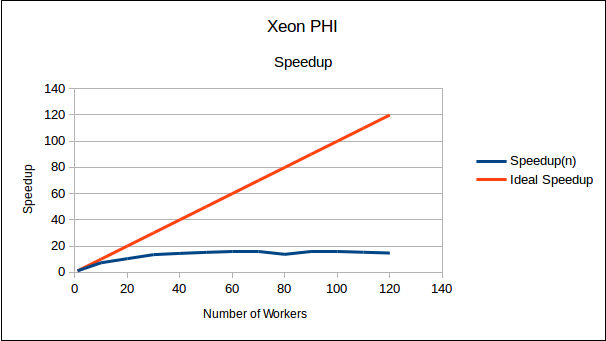
\includegraphics[scale=.75]{XeonPHI_Speedup.png}
	\caption{Speedup on the XeonPHI.}
	\label{fig:xeonphispeedup}
\end{figure}

\begin{figure} 
\centering
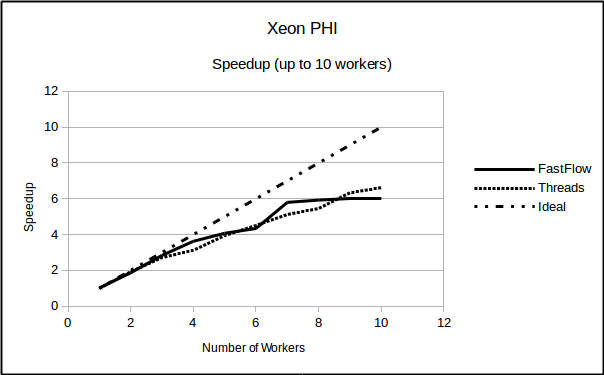
\includegraphics[scale=.75]{XeonPHI_Speedup10.png}
\caption{Scalability on the XeonPHI for the first 10 workers.}
\label{fig:xeonphispeedup10}
\end{figure}

\begin{figure} 
	\centering
	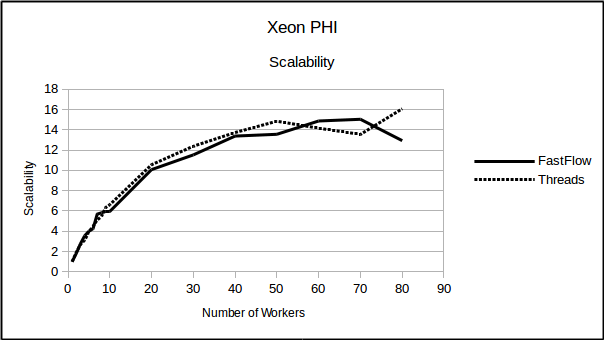
\includegraphics[scale=.75]{XeonPHI_Scalability.png}
	\caption{Scalability on the XeonPHI.}
	\label{fig:xeonphiscalability}
\end{figure}

\begin{figure} 
	\centering
	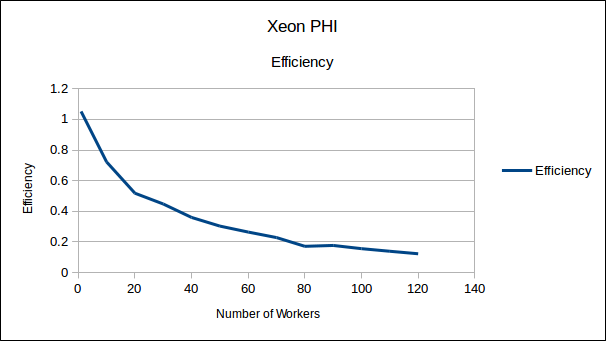
\includegraphics[scale=.75]{XeonPHI_Efficiency.png}
	\caption{Efficiency on the XeonPHI.}
	\label{fig:xeonphiefficiency}
\end{figure}

\end{document}

